\documentclass[a4paper]{article}
\usepackage{nips13submit_e}
%-------------
% SETTINGS
%-------------
    \usepackage{graphicx, subfig, float , multirow, array}
	\usepackage{amsmath, amsthm, amssymb, verbatim , stmaryrd}
    \usepackage{caption}
	\captionsetup{justification=centering, font=footnotesize, skip=1pt}
	\usepackage[left=2.4cm,right=2.3cm,top=2.4cm,bottom=2.3cm]{geometry}
	\usepackage{hyperref}
	\usepackage{fancyhdr}
    \pagestyle{fancy}
    \fancyhf{}
    \fancyfoot[L]{Confidential - Do not publish.} % change it to something else as you see fit.
    %\renewcommand{\sectionmark}[1]{\markboth{#1}{}}
    %\fancyfoot[R] {\thepage $|$ \leftmark}
    \fancyfoot[R] {page \thepage}
    \renewcommand{\headrulewidth}{0pt}
    \renewcommand{\footrulewidth}{1pt}
    \graphicspath{{figures/}}
	%\setlength{\parindent}{0cm}
	\renewcommand{\baselinestretch}{1.2}
%-----------------------
% TIKZ
% -----------------------
    \usepackage{tikz}
    \usetikzlibrary{arrows,positioning}
    \tikzstyle{state}=[draw, fill=white, align=center]
    \tikzstyle{sum}=[draw, circle, fill=white, align=center, inner sep=1,outer sep=0]

%------------------------
% MATH
% -----------------------
	\newcommand{\p}{\mathbb{P}}
	\newcommand{\Q}{\mathbf{Q}}
	\newcommand{\W}{\mathbf{W}}
    %\renewcommand{\theequation}{Eq\arabic{equation}}


%-------------
% TITLE
%-------------
	\author{Maha Elbayad \\ \texttt{maha.elbayad@student.ecp.fr}  \And Simon Rodriguez \\
    \texttt{simon.rodriguez@student.ecp.fr} \AND Supervisor: \\Catherine Herold, Morpho \And ECP Supervisor: \\Nikos Paragios, CentraleSupelec}
	\title{Glasses detection using CNN\\ECP 3rd year project}
	\date{}
%------------------------
% CONTENT
% -----------------------

\nipsfinalcopy %comment to add numbering 

\begin{document}
\maketitle
\begin{abstract}
    The performance of Convolutional neural networks depends on the amount of labeled samples and their presumable quality, i.e. having correct labels that are suited to the tackled problem. Since hand labeling is impractical on large databases, a shift toward semi-automatic labeling is inevitable, which means less accurate and sometimes misleading data that must be handled differently. We consider here the problem of binary classification with respect to the presence or not of glasses on a face. In this context, we will have to handle the presence of image dependent noise (labels are obtained by an existing imprecise classifier) and we attempt to assess the noise level present in the training set during the preprocessing and/or while learning. 
\end{abstract}

\section{Introduction}
    With the rise of deep learning and the improved ability to build huge datasets extracted from multiple sources, CNN classifiers can be designed and trained to perform complex tasks. Their accuracy and precision improve upon what could be achieved with conventional machine learning methods. Convolutional neural networks have shown to be surprisingly efficient on complex pattern recognition tasks, notably image classification \cite{krizhevsky2012imagenet}. But as the datasets grow bigger, it becomes harder to have ground-truth labels associated with the training data. When hundred of thousands of samples are collected in a semi-automated fashion, hand-labeling them is a task too time-consuming to be accomplished at a reasonable cost. Automatic annotation is used to obtain labels in a faster way: this labeling can rely on multiple techniques (image processing, simpler machine learning models, ...) with variable degrees of accuracy. These methods introduce labeling errors in the training set, ie. a source of noise that the classifier will have to deal with during its learning phase. Such noise results from multiple sources, among others, random errors, bias in the annotator and quality of the samples\cite{xiao2015learning}, and can disturb or decrease the performances of the classifier \cite{flatowrobustness}.
    Handling this noise in a supervised or semi-supervised setting is a currently active field of research due to the reasons presented above. Most of the methods studied can be separated in two groups: preprocessing of the noise through filtering of the dataset, and accounting for the noise in the structure of the classifier itself \cite{frenay2014comprehensive}.

    Preprocessing methods range from simple thresholding that reproduce an observed noise repartition to more complex setups where specific assumptions on the sources of noise are made \cite{frenay2014classification}. Other techniques focus on training a first classifier using a small hand-labeled subset as a reference, designed to predict the level of noise of a given sample. The dataset is relabeled using this classifier before training a standard CNN.

    In the second group, methods were introduced which implement new activation layers designed to handle noisy samples, for example: uncertain neural network for uncertain data classification called UNN\cite{ge2010unn}, surrogate losses functions that distinguish between samples taken from a hand-labeled subset and samples with noisy annotations \cite{NIPS2013_5073} and the use of multiple labels generated in a preprocessing pass where new labels are built to denote the probabilities that a sample falls within a class of noise (e.g. noise free, pure random noise or confusing noise) , these probabilities can then be combined to tune another classifier during the training phase \cite{xiao2015learning}.
    The introduction of a confusion matrix, either designed from observations on the dataset or learned during the training phase of the classifier \cite{Sukhbaatar:Qk8RHYrX}, follows a similar logic: the confusion matrix is fixed during a first step of the training, and is unconstrained during a second learning step.
    %These methods require various degrees of knowledge on the noise observed in the dataset, something that is not always possible or wished. 
    Each of these methods makes different assumptions on the noise distribution: the noisy labels are either assumed independent of the true label \cite{larsen1998design} or dependent on the true label but conditionally independent with the image\cite{Sukhbaatar:Qk8RHYrX} which is unrealistic and ill-suited to confusing labels related to some challenging samples. 
    To avoid any noise modeling, more general methods of performance enhancements from the machine learning field can be transposed to our subject. Bootstrapping was especially studied, where a combination of the initial training labels and the current classifier’s predictions are combined to generate new labels for the next training iteration \cite{Reed:MnuVRqvK}.

    %[x] to finish (S)
    %[x] proofreading the intro (M)
     
    % [x] Introduce the sections(M)
      
    In the first two sections of this report we lay out our general experimental setting and the chosen baseline model. In section \ref{sec:4} we list our evaluation criteria and analyze some dataset statistics that might interfere with the model performance before describing the methods we investigated in the course of this project: first with two major preprocessing methods, limiting the noise level through dataset preprocessing (section \ref{sec:preprocessing}) and noise cleansing with a classifier trained on a small clean dataset (section \ref{sec:cleansing}). Then, from the second group of methods we focused on the confusion matrix technique\cite{Sukhbaatar:Qk8RHYrX}(section \ref{sec:Qmatrix}) before introducing some bootstrapping schemes (section \ref{sec:bootstrap}). 

\section{Setting}

	\subsection{Caffe}
	We use the Caffe framework \cite{jia2014caffe} developed by the Berkeley Vision and Learning Center to train and test our neural networks. The framework relies on a pure C++/CUDA architecture, allowing for good performances when run on GPU. Bindings with Python and Matlab are provided but we generally used the direct command-line interface, as the main learning phase took place on the Ecole CentraleSupelec computing center, on a node equipped with two 12 cores Intel Xeon E5‐2695v2 (2.4Ghz) and a Nvidia Tesla K40 GPU. Caffe relies on a text file based definition for networks and configuration, allowing us to quickly define multiple tests.
		
	\subsection{Dataset}
	We experiment with the CASIA WebFace database~\cite{yi2014learning} containing 380,000 face images of about 10,000 subjects semi-automatically collected from the internet, mainly the IMDB website. We hand-labelled 4661 images from the CASIA database for validation (denoted \texttt{Test}) and another 4152 images for clean training (denoted \texttt{Tr1}) the rest (denoted \texttt{CASIA}) is labelled with an glasses detector based on edges information, especially the presence of the bridge of the glasses between the two eyes. The scores of the detector range from 0 to 255 and their distribution given the true label of an input image on manually annotated databases is shown in figure \ref{bench}. (Those databases being confidential, we cannot display examples of pathological cases where images are mislabelled.)
	
	%[x] Corriger les labels, anonymiser les résultats, afficher la même chose sur Tr1, Tr2 et Test
    % Je ne dispose pas des labels de Tr2
    % Ah oui c'est vrai, sorry.
    %[x] préciser que les datasets sont confidentiels et qu'on ne peut donc pas diffuser les images
    %[x] ajouter images de CASIA (vérifier les clauses)
	\begin{figure}[H]
	    \centering
	    \includegraphics[width=17cm]{old_classifier/benchmark}
	    \caption{Scores distribution on benchmark datasets\label{bench}}
	\end{figure}
    \begin{figure}[H]
        \centering
        \includegraphics[width=12cm]{old_classifier/benchmark_trte}
        \caption{Scores distribution on subsets Tr1 and Test \ref{datastat}}
    \end{figure}
    We can evaluate the performance of the old classifier, using indicators that will be described in further details in section \ref{eval_crit}. If we threshold the scores obtained on the test set via the old classifier at some point $t$ we can assess the classifier performance. When varying the threshold $t$ we notice that we can balance the trade-off between precision and recall at a threshold of 26 (figure \ref{tradeoff}). At this exact threshold, 5\% of the images from \texttt{CASIA} would be considered positive (with glasses). This ratio of 5\% is also obtained on randomly sampled subsets from \texttt{CASIA} that we hand-labeled which means that our dataset is initially skewed and unbalanced.

    In the following sections we will refer to the performance of the existing classifier as \texttt{perfOld}.
	%[x]bouger les figures dans la partie "Mesure de perfs" (je les duplique déjà)+images de cas difficiles (les enlève-t-on d'ici ?)
	\begin{figure}[H]
    \centering
    \subfloat[ROC curve]{\includegraphics[height=4cm]{old_classifier/roc}}
    \vspace{5pt}
    \subfloat[Precision-Recall curve]{\includegraphics[height=4cm]{old_classifier/pr}}
    \vspace{5pt}
    \subfloat[Precision \& recall curves\label{tradeoff}]{\includegraphics[height=4cm]{old_classifier/pr_th}}
    \caption{Performance of the existing classifier}
	\end{figure}
	We enriched our training set with 4151 images\footnote{courtesy of the multimedia lab in Hong Kong (\texttt{http://mmlab.ie.cuhk.edu.hk/projects/TCDCN.html})} manually labelled (denoted \texttt{Tr2}) that have higher image quality and less compression artifacts with a positives ratio of 20\%. We denote with \texttt{Tr3} the fusion of \texttt{Tr2} with a balanced subset of \texttt{Tr1} (1070 images) to maintain the 20\% positives ratio. The datasets statistics are shown in table \ref{datastat}, namely the dataset size, the number of its positive samples (with glasses) and the positives ratio, that is the percentage of the positive samples (with glasses) to the whole dataset, denoted by $r$.
	\begin{table}[H]
	\centering
	\begin{tabular}{|c|c||c|c|}
	\hline
	Set            & \#images & \#with glasses  & $r$\\
	\hline
	\texttt{CASIA} & 381949   &     unknown         &  unknown     \\
	\texttt{Test}  & 4661     &     246         &  5.3\%   \\
	\texttt{Tr1}   & 4152     &     214         &  5\%     \\
	\texttt{Tr2}   & 4151     &     789         &  19\%    \\
    \texttt{Tr3}   & 5221     &     1003        & 19.21\%\\
	\hline
	\end{tabular}
	\caption{Datasets statistics\label{datastat}}
	\end{table}

\section{The baseline model architecture\label{baseline}}%[x] lien vers autre architecture (elle doit nous l'envoyer par mail)
    Our model is inspired by the Alexnet architecture and the CNN architecture described in \cite{net1} and refined in \cite{net2}, with 3 blocks of convolution, ReLU and max-pooling layers followed by 2 fully-connected layers whose output for the sample $x_n$, $(\mathit{fc}_{n,k})_{1\leq k\leq K=2}$ is fed to a softmax loss i.e. we minimize the multinomial logistic loss over the whole training set $\mathcal X=\{x_n,y_n\}_{1\leq n\leq N}$:
    \begin{equation}
    \label{loss}
    \mathcal L(\mathbf W)=-\frac{1}{N}\sum_{i=1}^N\log(\hat p_{n,y_n}),\phantom{abc}\hat p_{n,k}=\frac{\exp(\mathit{fc}_{nk})}{\sum_k\exp(\mathit{fc}_{nk})}
    \end{equation}
    We denote with $\W$ the weights of the network. The regularization is assured with dropout on the fully-connected layers. The hyperparameters of the architecture are summarized in table \ref{params}.
    \begin{table}[H]
    \centering
    \begin{tabular}{|c|c|c|c|}
    \hline
    Layer name & type                    & Filter size/stride & output size $(N \times C \times H \times W)$\\
    \hline
    Conv1      & convolution             & 3x3/1              & 64 32 96 96\\       
    ReLU1      & & &\\
    Pool1	   & Max pooling             & 2x2/2              & 64 32 48 48\\
    \hline
    Conv2      & convolution             & 3x3/1              & 64 64 48 48\\       
    ReLU2      & & &\\
    Pool2	   & Max pooling             & 2x2/2              & 64 64 24 24\\
    \hline
    Conv3      & convolution             & 3x3/1              & 64 128 24 24\\       
    ReLU3      & & &\\
    Pool3	   & Max pooling             & 2x2/2              & 64 128 12 12\\
    \hline
    FC1        & fully-connected         &                    & 64 512\\
    drop1      & Dropout (50\%)          & &\\
    ReLU4      & & &\\
    \hline
    FC2        & fully-connected         &                    & 64 2\\
    drop2      & Dropout (50\%)          & &\\
    \hline
    loss       & Softmax loss            &                    & 1 \\
    \hline
    \end{tabular}
    \caption{Baseline model hyperparameters\label{params} : N=Number/batch size, C=Channels, W=Width, H=Height}
    \end{table} 

    The general learning hyperparameters (learning rate, weight decay) were defined at the beginning of the project with the supervising team at Safran Morpho. In fact, the goal of the project was never to fine-tune a CNN or explore the space of its hyperparameters, thus those values were fixed once and for all (see \ref{cnn_param}).

\section{Experiments \& Results}\label{sec:4}
    During this study, we tried to follow two directions in our research and experimentations: the first one was to get the best classification possible, even if this implies to hand-label a subset of the initial dataset. This will be addressed in the first experiment, where we will show that this methodology can indeed lead to the best performances. The second axis aimed to take into account the fact that some labels are noisy. Even if the performances obtained on a noisy dataset are initially lower, a wider range of methods (as described in the first section) can be applied to improve the scores and bring interesting results.

    \subsection{Evaluation criteria}{\label{eval_crit}}
        \begin{minipage}{.7\textwidth}
        We start by presenting the main indicators we will rely on to assess the performances of our experiments. All our evaluators are using the \texttt{Test} dataset, and are based on the comparison between the ground truth labels and the scores output by the CNN on this set.
        For all the following definitions we consider the notations in the table to the right.
        \end{minipage}\hspace{10pt}
        \begin{minipage}{.2\textwidth}
        \begin{table}[H]
            \centering
            \begin{tabular}{cc|c|c|}
            \cline{3-4}
                & & \multicolumn{2}{c|}{prediction}\\
                \cline{3-4}
                & & 1 & 0\\
                \hline
                \multicolumn{1}{|l|}{\multirow{2}{*}{\shortstack{ground\\ truth}}}& 1 & tp & fn \\ 
                \cline{2-4}
                \multicolumn{1}{|l|}{}& 0 & fp & tn \\ 
                \hline
                \end{tabular}
        \end{table}
        \end{minipage}
        \begin{itemize}
        	\item \textbf{Accuracy:} The accuracy is the simplest indicator, defined as the ratio of the number of correct predictions over the number of samples tested. It only makes the distinction between erroneous and correct predictions, and is thus a very global indicator, that furthermore relies on the necessity to define a threshold on the scores given by the classifier ($accuracy = \dfrac{tp + tn}{tp + tn + fn + fp}$).
        	\item \textbf{Confusion matrix:} The confusion matrix enhance the concept of accuracy by discerning four cases: the true positives (tp), the true negatives (tn), the false positives (fp) and the false negatives (fn). It allows one to better grasp the behavior of the classifier ; depending on the desired application, a classifier that makes more false positives than false negatives can for instance be preferred.
        	\item \textbf{Receiver Operating Characteristic:} The ROC curve expresses the true positive rate, also called the sensitivity, equal to $\dfrac{tp}{tp+fn}$, as a function of the false positive rate, also called the fall-out, i.e. $\dfrac{fp}{fp+tn}$. Each point of the curve is obtained by setting a threshold on the scores of the classifier (i.e. the output of the softmax layer of the CNN) and computing the corresponding ratios.\\
        		Any ROC curve will pass through the points (0,0) and (1,1) as they corresponds to the points where all samples are negative/positive respectively. A random classifier will have the identity line as a ROC curve, while a perfect classifier ROC is composed of the lines from (0,0) to (0,1) and from (0,1) to(1,1).\\
        		By choosing a false positive rate corresponding to the behavior of the desired classifier, one can assess how well it performs at this given rate. 
    		%[x]any idea for a better explanation ?
    		% May be you could mention that each point (tpr,fpr) comes from choosing a threshold of the scores
    		% Any roc curve passes through (0,0) and (1,1) = all samples are negatives or all samples are positives
    		%Thanks, I'll add this
        	\item \textbf{Area Under the Curve:} The area under the ROC curve is equal to the probability that the classifier will predict a higher label for a randomly chosen image labelled 1 than for another randomly chosen image labelled 0. 
        	\item \textbf{Precision-Recall:} The PR curve expresses the precision (the number of ground truth positive correctly defined as positive by the classifier, divided by the total number of images labelled as positive by the classifier) as a function of recall (the number of ground truth positive correctly defined as positive by the classifier, over the total number of images that really are labelled positives). A higher precision implies that the classifier gives positive labels in a relevant way (not too many false positives), while a high recall means that the classifier detects positives more efficiently (not too many false negatives).\\
        	Using the notations of the table above, we have that precision = $\dfrac{tp}{tp+fp}$ and recall = $\dfrac{tp}{tp+fn}$.
            % \begin{table}[H]
    		% \centering
    		% \begin{tabular}{|l|l|l|}
    		% \hline
    		% 	\backslashbox{Ground truth}{Prediction} & 1  & 0  \\ \hline
    		% 	1 & tp & fn \\ \hline
    		% 	0 & fp & tn \\ \hline
    		% 	\end{tabular}
    		% \end{table}
            
    		%[x]add table and explanation 
    		
        	\item \textbf{Average precision:} This is the area under the PR curve. It gives a general overview of the PR behavior of the classifier.
        \end{itemize}
        In the figure below the performances curves of the original classifier are shown, along with the numerical evaluators described above.
        \begin{figure}[H]
        \centering
        \subfloat[ROC curve]{\includegraphics[height=4cm]{old_classifier/roc}}
        \vspace{5pt}
        \subfloat[Precision-Recall curve]{\includegraphics[height=4cm]{old_classifier/pr}}
        \caption{Performances of the existing classifier:\\Accuracy=0.962, AUC=0.920, Average Precision=0.679}
    	\end{figure}

    \subsection{The effects of the training set statistics}
        \subsubsection{The positive samples ratio}
       
            We train our model on the sets \texttt{Tr1}, \texttt{Tr2} and \texttt{Tr3} respectively and evaluate each model on the \texttt{Test} set. \texttt{Tr1} share the same distribution as the test set ($r\approx 5\%$) while \texttt{Tr2} have more positive samples ($r\approx 20\%$) and so does \texttt{Tr3} with more samples to train on. The results in figure \ref{perfX} show that the CNN underperforms when the training data is skewed, i.e. the two classes are unbalanced (the performance of \texttt{Tr2} compared to \texttt{Tr1}), as it tends to promote the more frequent class. The fact that \texttt{Tr1} and \texttt{Test} are drawn from the same sample may favor training with \texttt{Tr1} but balancing the training set by means of under-sampling~\cite{drummond2003c4} or optimizing a class-sensitive cost~\cite{NIPS2013_5073}\cite{elkan2001foundations}\cite{zhou2006training} yields better results.

            We approached the cost sensitivity by training our baseline model with a different loss function built on the cost matrix $\mathbf C$, where:
            \[
            \mathbf C = 
            \begin{pmatrix}
            c_{00}&c_{01}\equiv c_{FN}\\
            c_{10}\equiv c_{FP}&c_{11}
            \end{pmatrix}
            \]
            $c_{i,j}\equiv$ the cost of predicting $i$ when the ground truth is $j$.\\
            To implement this new loss function in \textit{Caffe} we adapt the already existing \texttt{InfoGainLoss} layer which inherits from the multinomial logistic loss (\ref{loss}):\\
            \[\mathcal {\tilde L}=-\frac{1}{N}\sum_i\left(H_{y_n,0}.\log\hat p_{n,0}+H_{y_n,1}.\log\hat p_{n,1}\right)\]
            To achieve proportional misclassification costs to the ones defined in $\mathbf C$ we set:
            \[H = 
            \begin{pmatrix}
            c_{01}&c_{00}\\
            c_{11}&c_{10}
            \end{pmatrix}\]
            On figure \ref{unbLoss}, $c_{01}$ is the cost of a false negative, the image of $\p(y=1)=0$ on the positive curve (to the extreme left) and $c_{10}$ is the cost of a false positive, the image of $\p(y=1)=1$ on the negative curve (to the extreme right).\\
            Intuitively, we would want for the misclassification costs $c_{10}$ and $c_{01}$ to satisfy $c_{10}\p(y=0) : c_{01}\p(y=1)$ and for the correct classifications to have a zero cost. $H1$, and to a lower extent $H2$, were defined with this objective in mind. $H3$ takes the opposite direction with a false negative cost slightly lower than the false positive cost. 
            \begin{center}
            \begin{minipage}{.6\textwidth}
            \begin{figure}[H]
                \centering
                \includegraphics[width=6cm]{exp1/losses}
                \caption{Loss function per cost matrix\label{unbLoss}}
            \end{figure}
            \end{minipage}
            \begin{minipage}{.3\textwidth}
            $
            H1 = \begin{pmatrix} 1 & 0 \\ 0 & 0.05 \end{pmatrix}\\ %Q16
            \phantom{abc}\\
            H2 = \begin{pmatrix} 0.95 & 0 \\ 0 & 0.2 \end{pmatrix}\\ %Q15
            \phantom{abc}\\
            H3 = \begin{pmatrix} 0.95 & 0 \\ 0.05 & 1 \end{pmatrix}\\ %Q13
            $
            \end{minipage}
            \end{center}
            \begin{figure}[H]
            \centering
            \subfloat[Log ROC]{\includegraphics[height=5cm]{exp1/unb1}}
            \subfloat[ROC zoom-in]{\includegraphics[height=5cm]{exp1/unb2}}
            \subfloat[ROC zoom-in\label{6c}]{\includegraphics[height=5cm]{exp1/unb3}}

            \caption{Roc curves with the 3 different losses compared to the default softmax loss - \texttt{Tr1}}
            \end{figure}

            The model with $H1$-loss performs marginally better than the softmax model with a lower precision yet on the ROC curve it achieves higher true positives rate (northeast of the ROC figure \ref{6c}) i.e. low false negatives rate which is coherent with the higher false negative cost assigned (1 vs. 0.05). $H2$ is slightly equivalent to the softmax model. $H3$ on the other hand performs surprisingly well, one possible interpretation is that most classifiers assign a zero cost to correctly classifying a sample $(c_{00}=c_{11}=0)$, however, with $H3$ the classifier is encouraged to doubt the class of all samples with a lower cost at $p(y=1)=0.95$. Such costs have a regularization effect on the model.

            The best performances on \texttt{Tr1}, \texttt{Tr2} and \texttt{Tr3} were achieved with the following parameters:
            \[H_{Tr2}=H_{Tr3}=\begin{pmatrix}0.99&0.01\\0.2 & 0.8\end{pmatrix}\]
            \[H_{Tr1}=\begin{pmatrix} 0.95 & 0 \\ 0.05 & 1 \end{pmatrix}\]

            %[x] présenter la matrice 'dans l'autre sens'
            %[~] a commenter d'avantage
            %[~] référence article
                
            %[x] Souligner que c'est bien le cas bien que Tr1 soit directement extrait de la même base que test, avec la même proportion (ie avoir + d'images est + important qu'avoir la bonne repartition)
            %[!] En conclusion, mettre en avant l'importance d'un certain equilibre entre les classes (Not sure about this!) (Oui du coup avec les derniers résultats ca n'est plus si evident)
            %[x] Préciser les formule de la fonction de cout pour montrer le changement
            %[x] Tester modif de la fonction de cout sur Tr2 pour voir si meilleur resultat
            
            We will refer to the model trained on \texttt{Tr3} with $H_{Tr3}$ as \texttt{perfTr3} and we may refer as well to the best performance achieved on $\texttt{Tr1}$ as \texttt{perfTr1} and that on $\texttt{Tr2}$ as \texttt{perfTr2}.
            \begin{figure}[H]
                \centering
                %\includegraphics[height=4.5cm]{exp1/perfX} %[x] Add perftr2
                %\includegraphics[height=5cm]{exp1/clean_roc_balance}
                \includegraphics[height=5.5cm]{exp1/perfXroc}
                \includegraphics[height=5.5cm]{exp1/perfXpr}
                \caption{Best performance on each training set\label{perfX}}
            \end{figure}
            
				%[x] impact sur ROC complète
        \subsubsection{The training set size}
            In this section we experiment with varying the training set size to determine the optimum size necessary to achieve better performance in two different modes: with clean labels and with noisy labels induced from the existing classifier.

            All the models below are trained with the softmax default loss described in section \ref{baseline}. For the clean datasets, we start with \texttt{Tr3} and we keep decreasing the dataset size iteratively in order to build nested training sets.
			%[x] préciser qu'on travaille de nouveau avec la loss habituelle
            % \begin{table}[H]
            % %\centering
            % \textbf{Clean labels:}\\%<-[x] quelles bases utilisées ?
            % \begin{tabular}{|c|c|c|c|c|c|c|c|c|c|c|}
            % \hline
            % size & 5221 &4708 &3809 &2843 &1880 &1116 &583 &265 &118 &36 \\
            % \hline
            % $r$& 19\% &19\% &19\% &19\% &18\% &17\% &16\% &15\% &14\% &19\%\\
            % \hline
            % \end{tabular}\\
            % \begin{tabular}{|c|c|c|c|c|c|c|c|c|c|c|c|}
            % \hline
            % size & 4152 & 3800 & 3400 & 3000 & 2500 & 2000 & 1600 & 1300  & 1000  &600 & 400 \\
            % \hline
            % $r$ & 5\% &  5\%  &5\% &   5\%  &  5\%   & 5\%  & 5\%   & 6\%  &  5\%   & 6\%  & 5\% \\
            % \hline
            % \end{tabular}\\

            % \vspace{5pt}
            % \textbf{Noisy labels - scores binarized for 7.5\% positive samples:}\\%[x] Ressortir sur une base bruitée avec 20% de positifs
            % \begin{tabular}{|c|c|c|c|c|c|c|c|c|c|c|c|}
            % \hline
            % size & 2k & 5k & 10k & 20k & 50k & 100k & 150k & 200k & 250k & 300k & 350k \\
            % \hline
            % $r$ & 7\% & 8\% &8\% & 7\% & 8\% & 7\% &7\% & 7\% &7\% &7\% &7\%\\
            % \hline
            % \end{tabular}
            % \begin{tabular}{|c|c|c|c|c|c|c|c|}
            % \hline
            % size & 1k & 2k & 5k & 10k & 20k & 50k & 100k \\
            % \hline
            % $r$ & 23\% & 25\% &21\% & 22\% & 22\% & 20\% &20\%\\
            % \hline
            % \end{tabular}
            % \end{table}
		
            \begin{figure}[H]
                \centering
                \includegraphics[height=6cm]{exp1/roc_size}
                \caption{A selection of roc curves with different sizes, modes (clean/ noisy) and ratios $r$\label{rocsize}}
            \end{figure}
            %[x]Faire figurer clean 5221 (encore meilleur)
            %{x]Commenter les differences entre les clean à size constante
            %[x]Ajouter courbe noisy 20% 100000
			%
            We note that the training set size is more impactful when the labels are clean, in fact:\\
            \textbf{Clean labels:}
            \begin{itemize}
            \item The average precision and the area under the ROC curve (AUC) strongly increase with the dataset size at fixed positives ratio : $r=20\%$: $(2)\rightarrow (1)$ and  $r=5\%$: $(4)\rightarrow (3)$.
            \item The average precision and the area under the ROC curve (AUC) increase with the ratio of the observed positive samples at a fixed size : size $\approx 2000$: $(4)\rightarrow (2)$.
            \end{itemize}
            \textbf{Noisy labels:}
            \begin{itemize}
            \item The training set size seems to have little to no effect on the performance:  $r=5\%$: $(7)\rightarrow (6)$ then $(6)\rightarrow (5)$ and $r=20\%$: $(8)\rightarrow (9)$.
            \item the positives ratio is ineffective too with a fixed size : size = 2000 : $(8)\rightarrow (7)$
            \end{itemize}
            
            %[x] bullet points pour les interpretations
            \begin{figure}[H]%Ajouter l'ancien detecteur
                \centering
                \includegraphics[width=12cm]{exp1/ap_auc}
                \caption{Performance with different sizes and different $r$: clean vs noisy}
            \end{figure}
			% Expliquer comment la base noisy 20% est créee.
            % [x] Something is off with the 100k test (On which dataset ? noisy20pc ? I can check the lmdb and rerun it if you want)
            % [x] A commenter: de manière séparée bruit/clean, pour montrer l'impact du nombre d'ex.
            % [x] diff 5%/20% en clean, en noise. Commenter peu de gain 5%/20% sur noisy, puis clean vs noise.
            % [x] Entre les deux, pour le même nombre d'ex. (et même %)
            
    \subsection{Limiting errors through dataset preprocessing}\label{sec:preprocessing}
        We now experiment with the whole \texttt{CASIA} base (minus the \texttt{Test} set), to study how the scores from the old classifier can be binarized. We adopt a simple model, where a threshold $t$ is fixed : all images with a score lower than $t$ are labelled 0, all images with a score higher than $t$ are labelled 1. The binarization implies a loss of granularity compared to the raw scores of the old classifier, but is needed due to the structure of the CNN. A basic threshold applied as described above is a simplifying model, as it will mislabel the pictures that were outliers for the old classifier, introducing the same type of error during the learning phase; for those images, we expect that the picture itself will contain enough information for the CNN to rectify the mistakes.
        
        \subsubsection{Varying the threshold\label{vary:th}}
            We select thresholds based on the percentage of labels 1 that we want to have in our training set, of total size approx. 381000.
            \begin{table}[H]
            \centering
            \label{table_th}
            \begin{tabular}{|l|l|l|l|}
            \hline
            Threshold & Corresp. score & \#with glasses & AUC   \\ \hline
            2.5\%    & 41.5  & 9549           & 0.934 \\ \hline
            5\%      & 26.7  & 19098          & 0.938 \\ \hline
            7.5\%    & 21.2  & 28647          & 0.954 \\ \hline
            10\%     & 18.4  & 38195          & 0.944 \\ \hline
            \end{tabular}
            \caption{Repartition and AUC for each threshold. }
            \end{table}
            
            \begin{figure}[H]
                \centering
                \subfloat[ROC curves]{\includegraphics[height=6cm]{figures/th_and_margin/rocs_th}}
                \vspace{5pt}
                \subfloat[ROC curves (zoom)]{\includegraphics[height=6cm]{figures/th_and_margin/rocs_half_th}}\\
				\subfloat[ROC log curves]{\includegraphics[height=6cm]{figures/th_and_margin/rocs_log_th}}
                \vspace{5pt}
                \subfloat[Precision-Recall curves]{\includegraphics[height=6cm]{figures/th_and_margin/recall_th}}
                \caption{Impact of the binarization threshold on the classification performances}
                 \label{fig:thfig1}
            \end{figure}
			%[x] figure à inverser
            We observe in figure \ref{fig:thfig1} that the network performances degrade if the threshold is set high, as the numbers of pictures in each class are unbalanced. The best threshold seems to lie a bit above the empirical threshold of 5\% (score=26.7), corresponding to the repartition observed in the hand-labelled datasets. At 7.5\%, we allow for images with glasses that were given a lower score by the old classifier to be correctly identified by the CNN. This is also an indication that a step of data augmentation in order to balance the two classes could improve the performance. The question of the selection of the duplicated pictures based on the noisy labels remains open.

        \subsubsection{Introducing a margin}

            We furthermore introduce a notion of rejection margin around the threshold, where we discard all images that have a score $s$ such that $|s - t| \leq m$. The rationale is that for these pictures, the score from the old classifier is unsure and should thus be ignored. We select a binarisation threshold of 5\% in order to stay close to the observed distribution of the true labels. When the margin gets larger, the size of the training set decreases, an effect that has consequences on the performances if this size becomes too small : once again the two classes are unbalanced, and the outliers mis-labelled by the old classifier have more influence on the results.

            \begin{table}[H]
            \centering
           
            \begin{tabular}{|l|l|l|l|l|l|}
            \hline
            m & \#images & \#with glasses & $r$ & Accuracy at 10k it. & AUC   \\ \hline
            0      & 381949   & 19086          & 4.9\% & 0.9722              & 0.952 \\ \hline
            5     & 368956   & 14565          & 3.9\% & 0.9713              & 0.953 \\ \hline
            10     & 347032   & 11551          & 3.3\% & 0.9711              & 0.949 \\ \hline
            15     & 286729   & 9470           & 3.3\% & 0.9680              & 0.962 \\ \hline
            20     & 107152   & 7851           & 7,3\% & 0.8759              & 0.941 \\ \hline
            25     & 6630     & 6587           & 98\%  & 0.0878              &       0.699 \\ \hline
            \end{tabular}
            \caption{Repartition of labels and results for a variable margin}
            \label{table_margin}
            \end{table}
            Table \ref{table_margin} shows that as the margin increases, the general accuracy decreases. But depending on the operating point (fig. \ref{fig:marginfig1}), it is possible to get better results with a margin defined by $m=15$, where many uncertain pictures have been rejected, but at the same time the dataset remains of a sensible size.
            \begin{figure}[H]
                \centering
                \subfloat[ROC curves]{\includegraphics[height=7cm]{figures/th_and_margin/rocs_margin}}
                \vspace{5pt}
                \subfloat[Precision-Recall curves]{\includegraphics[height=7cm]{figures/th_and_margin/recall_margin}}
            \end{figure}
            \begin{figure}[H]
                \centering
                \subfloat[ROC log curves]{\includegraphics[height=7cm]{figures/th_and_margin/rocs_log_margin}}
             	\vspace{5pt}
             	\subfloat[ROC curves (zoom)]{\includegraphics[height=7cm]{figures/th_and_margin/rocs_half_margin}}
                \caption{Impact of the margin width used for labelling on the classification performances}
                \label{fig:marginfig1}
            \end{figure}
         
         
         The methods studied in the two previous experiments were mainly focused on addressing the issue of noise through preprocessing of data, either by using a small hand-labelled subset, or by binarizing the scores of the old classifier based on the statistics of the \texttt{CASIA} dataset. Meanwhile, the learning phase in itself was similar to a standard CNN training.\\
         In the next tests, we try to take the noise into account directly during the training phase, allowing for a better handling of those uncertain labels.
            %[x] Marquer separation ici entre preprocessing sur les datasets et maintenant prise en compte bruit dans le CNN 
            
    \subsection{Training on noisy labels with a confusion matrix} \label{sec:Qmatrix}
        Sukhbaatar et al.\cite{FB} introduced an extra noise layer into the model which maps the network outputs ($\p(y=1)$ and $\p(y=0)$) to  the noisy label distribution.
        We implemented an adapted version of their method in \textit{Caffe} that consists of two phases: (1) training a convolutional neural network on the noisy data, (2) finetune the network with an additional constrained linear layer that would mimic a confusion matrix to retrieve a prediction closer to the true labels. 
        % In a first part, we try to learn the confusion matrix and in a second part, we will instead evaluate it manually on a subset of the training base.
        %[x] dernière phrase -> la mettre en section 4.4.3, au moment de tester sur données réelles
        \subsubsection{Noise modeling}
        \begin{minipage}{.65\textwidth}
            Given a training set $\mathcal X=\{(x_n,y_n)\}_{1\leq n\leq N}$ where $y_n\in\{1...K\}$ is the true label of the entry $x_n$ in the contest of a K-multiclass classification. The additional noise layer has optimally for weights the confusion matrix $\Q$ defined as:
            \[\Q=(q_{ij})_{1\leq i,j\leq K},\:\forall i,j\in\{1,..K\}\:q_{ij}=\p(\tilde y=i|y=j),\]
            where $\tilde y$ is the noisy label. In other words $q_{ij}$ is the probability of the class $j$ being mistaken for class $i$

            By the sum rule we can evaluate the noisy label as:
            \[\p(\tilde y=i|x)=\sum_jq_{ij}\p(y=j|x)\]
        \end{minipage}\hspace{10pt}
        \begin{minipage}{.2\textwidth}
            \begin{figure}[H]
               \centering
               \subfloat[Phase 1\label{ph1}]{
                    \centering
                    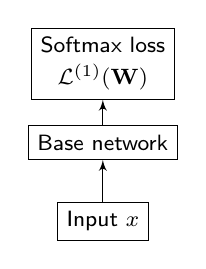
\begin{tikzpicture}[node distance=.5cm,auto,>=latex',font=\sffamily\footnotesize]
                        \node [state] (a) {Input $x$};
                        \node [state] (b) [above of=a,node distance=1cm] {Base network};
                        \node [state] (c) [above of=b,node distance=1cm] {Softmax loss\\$\mathcal L^{(1)}(\mathbf W)$};
                        \path[->] 
                        (a) edge node {} (b)
                        (b) edge node {} (c);
                    \end{tikzpicture}
                    } 
               \subfloat[Phase 2\label{ph2}]{
                    \centering
                    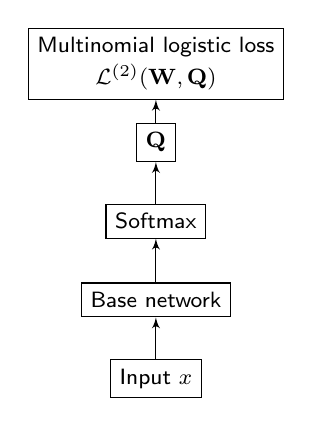
\begin{tikzpicture}[node distance=.5cm,auto,>=latex',font=\sffamily\footnotesize]
                        \node [state] (a) {Input $x$};
                        \node [state] (b) [above of=a,node distance=1cm] {Base network};
                        \node [state] (c) [above of=b,node distance=1cm] {Softmax};
                        \node [state] (d) [above of=c,node distance=1cm] {$\Q$};
                        \node [state] (e) [above of=d,node distance=1cm] {Multinomial logistic loss\\ $\mathcal L^{(2)}(\mathbf W,\Q)$};
                        \path[->] 
                        (a) edge node {} (b)
                        (b) edge node {} (c)
                        (c) edge node {} (d)
                        (d) edge node {} (e);
                    \end{tikzpicture}
                    }
                \caption{Model outline\label{outline}}
            \end{figure}
        \end{minipage}    
        \subsubsection{White noise - Case study}
            We introduce synthetic noise on the labels of \texttt{Tr1} with different levels $q_i$ on each class (0/1) then train the baseline model (fig \ref{ph1}) denoted noQ, as well as the model with the extra noise layer (fig \ref{ph2}) denoted w/Q on the noisy data. We can either learn $\Q$ in the second phase or simply infuse the true matrix evaluated on a clean subset of the training set. We tested both strategies:
            \paragraph{Learning $\Q$:}
            The learnt confusion matrix gets closer to the true matrix on its second column - class 1, while often converging to $(1,0)^T$ in its first column - class 0 given the skewed distribution of the labels (table \ref{learnQ}). Thus, the accuracy is weakly affected by the introduction of learnt $\Q$.
            \begin{table}[H]
                \centering
                \subfloat[]{
                \begin{tabular}{|cc|}
                \multicolumn{2}{c}{definition}\\
                \hline
                $1-q_0$ & $q_0$\\
                $q_1$ & $1-q_1$\\
                \hline
                \end{tabular}}
                \subfloat[$q_0=0.01, q_1= 0.19$]{
                \begin{tabular}{|cc||cc|}
                \multicolumn{2}{c}{Learnt Q}&\multicolumn{2}{c}{True Q}\\
                \hline
                1.00 & 0.20 & 0.99 & 0.19\\
                0.00 & 0.80 & 0.01 & 0.81\\
                \hline
                \end{tabular}}
                \subfloat[$q_0=0.02, q_1= 0.38$]{
                \begin{tabular}{|cc||cc|}
                \multicolumn{2}{c}{Learnt Q}&\multicolumn{2}{c}{True Q}\\
                \hline
                1.00 & 0.21 & 0.98 & 0.38\\
                0.00 & 0.79 & 0.02 & 0.62\\
                \hline
                \end{tabular}}
                \subfloat[$q_0=0.1, q_1= 0.01$]{
                \begin{tabular}{|cc||cc|}
                \multicolumn{2}{c}{Learnt Q}&\multicolumn{2}{c}{True Q}\\
                \hline
                1.00 & 0.06 & 0.90 & 0.01\\
                0.00 & 0.94 & 0.10 & 0.99\\
                \hline
                \end{tabular}}
                \caption{Confusion matrices: the learnt and the truly used to generate the noisy labels\label{learnQ}}
            \end{table}
            \paragraph{Evaluating $\Q$ on a subset:}
            This time, the introduction of the extra noise layer yields promising results as it can cope with high noise levels especially on the positive class (up to 57\%), but with high noise levels on the majority class (the negatives) the confusion matrix fails to handle the noise. 
            %[x]Matrice sur Q0 et Q1
            %[x]Changer le nom de "baseline"
            %[x] transformer la matrice en tableau :sigh ^^
            \begin{minipage}{.4\textwidth}
            \flushright
            \begin{tabular}{|c|c|m{2cm}|}
            \hline
            $q_0$ & $q_1$ & AUC\\
            \hline
            0.01 & 0.19  & $\text{noQ: } 0.9282$ $\text{w/Q: } 0.9552$\\
            \hline
            0.02  & 0.38  &$\text{noQ: } 0.8475$ $\text{w/Q: } 0.8962$\\
            \hline
            0.03  & 0.57  &$\text{noQ: } 0.7485 $ $\text{w/Q: } 0.8323$\\
            \hline
            0.1   & 0.01  &$\text{noQ: } 0.8927 $ $\text{w/Q: } 0.8959$\\
            \hline
            0.15  & 0.01  &$\text{noQ: } 0.8442 $ $\text{w/Q: } 0.8455$\\
            \hline
            0.2   & 0.02  &$\text{noQ: } 0.8381 $ $\text{w/Q: } 0.8437$\\
            \hline
            \end{tabular}
            \end{minipage}\hspace{20pt}
            \begin{minipage}{.4\textwidth}
            \begin{figure}[H]
            \centering
                \includegraphics[height=6cm]{figures/exp3/roc}
                \caption{Confusion matrix Roc-curves with white noise}
            \end{figure}
            \end{minipage}
            
            %[!] perfTr1 avec quelle loss ? (je sais pas si c'est vraiment necessaire de repréciser ca là ) 
            %[x]Petite analyse/conclusion comme quoi ca marche de ouf
            

        \subsubsection{Image dependent noise}
            If the model described above doesn't assume symmetric label noise (noise independent of the true label) it still does assume that the noise is independent of the input $x$, which is the case when binarizing the old classifier scores to label the training set; the existing classifier is based on gradient information strongly correlated with the glasses frame (low performance on recognizing rimless glasses) and is considerably sensitive to the contrast changes. 

            To challenge the confusion matrix method, we binarize the labels in 4 configurations with parameters $(t_0,t_1)$ such that the image is labelled 0 if the score is smaller than $t_0$ and labelled 1 if it is larger than $t_1$. We consider the full training set \texttt{CASIA} and we estimate the $\Q$ matrix on a subset of the training set (in this case samples from \texttt{Tr1} that are still remaining in the training set)
            %[x] ajouter # samples, proportion
            \begin{table}[H]
            \centering
            \begin{tabular}{|c|c|c|c|c|c|}
            \hline
            Test & $t_0$ & $t_1$ & \#images & \#with glasses & $r$\\
            \hline
            1 & 10  & 30 & 250341 & 15827 & 6.32\%\\
            2 & 20  & 20 & 381916 & 32132 & 8.41\%\\
            3 & 30  & 30 & 381942 & 15827 & 4.14\%\\
            4 & 40  & 40 & 381947 & 10079 & 2.64\% \\
            \hline
            \end{tabular}
            \end{table}
            For each training set, the estimated confusion matrix $Q_i$ on \texttt{Tr1}$\cap$\texttt{Training\_set}$_i$ are shown in figure \ref{rocQ}. Although the estimated matrices are quite similar to the white noise matrices (low $q_0$ and a large of $q_1$), in this context of image dependent noise, the method fails to improve the classification performance.
            \begin{figure}[H]
            \hspace{80pt}
            \begin{minipage}{.3\textwidth}
                $Q_1=\begin{pmatrix}0.98&0.02\\0.08&0.92\end{pmatrix}$\\
                $Q_2=\begin{pmatrix}0.95&0.05\\0.21&0.79\end{pmatrix}$\\
                $Q_3=\begin{pmatrix}0.997&0.003\\0.40&0.60\end{pmatrix}$\\
                $Q_4=\begin{pmatrix}0.995&0.005\\0.54&0.46\end{pmatrix}$\\
            \end{minipage}
            \begin{minipage}{.7\textwidth}
                \includegraphics[width=6cm]{exp3/iroc_zoom}
            \end{minipage}
            \caption{Q-matrix performance on image dependent noise\label{rocQ}}
            \end{figure}
            %[x]Expliquer pourquoi l'introduction de Q ne résout pas le problème
    \subsection{Bootstrapping methods}\label{sec:bootstrap}
        \subsubsection{Bootstrapping at a fixed positives ratio}\label{strap1} % I couldn't find a good title :p (M) Basic Bootstrapping for Beginners ? :p
            Another method we studied was the process of bootstrapping. We first focused on its simplest form, where: 
            \begin{enumerate}
            	\item the CNN is trained on a subset of \texttt{CASIA} with 20\% of positive samples (detailed below). %[x] detail the construction of the subset
            	\item the resulting network is then used to output new scores for the pictures of the training set.
            	\item the training set is re-labelled based on the new scores, by choosing a threshold that ensures 20\% of the pictures are labelled 1.
            	\item This process is iterated, and we track the evolution of indicators through the experiment.
            \end{enumerate}
            %[x] numbers instead of bullets
             We work on a subset of 100k pictures of \texttt{CASIA}, balanced at 20\% of positive labels, as this balancing has been shown to provide a better baseline in previous experiments. To build this set, we first binarize the scores of the \texttt{CASIA} images using the "natural" 5\% threshold described earlier. We then sample 20k images from the pictures labelled as 1 in the previous step, and 80k images from the ones labelled as 0.\\
            The third step was introduced as a way of regularizing the training set: if no ratio was imposed, the number of pictures labelled 1 could decrease with each iteration until the classifier learns to output only 0 labels.\\
            From one iteration to the next, we also keep track of the number of labels switched, shown below.\\
           We notice fluctuations from an iteration to the next, with an overall small improvement to AUC and ROC shape. The initial set is probably still too unbalanced to allow for bootstrapping to improve the performance. We see that from an iteration to the next, the number of labels switched is decreasing, implying that the network is converging to some set of parameters. But the gain in performance is small, and calls for the use of finer bootstrapping methods.
                 
            \begin{table}[H]
            \centering

            \label{table-bootstrap-simple}
            \begin{tabular}{l|l|l|}
            \cline{2-3}
                                               & \begin{tabular}[c]{@{}l@{}}\#modified labels wrt\\  previous iteration\end{tabular}  & AUC   \\ \hline
                                               
            \multicolumn{1}{|l|}{It 0 (old classifier)}          & 0         & 0.920 \\ \hline
            \multicolumn{1}{|l|}{It 1}         & 4892        & 0.953 \\ \hline
            \multicolumn{1}{|l|}{It 2}         & 1582    & 0.949 \\ \hline
            \multicolumn{1}{|l|}{It 3}         & 1184         & 0.955 \\ \hline
            \multicolumn{1}{|l|}{It 4}         & 828       & 0.953 \\ \hline
            \multicolumn{1}{|l|}{It 5}         & 800         & 0.955 \\ \hline \hline
            \multicolumn{1}{|l|}{\texttt{perfTr2}} & -         & 0.991 \\ \hline
            \end{tabular}
            \end{table}

            \begin{figure}[H]
                \centering
                \subfloat[ROC curves]{\includegraphics[height=6.5cm]{figures/bootstrap/roc_simple.pdf}}
                \vspace{5pt}
                \subfloat[Precision-Recall curves]{\includegraphics[height=6.5cm]{figures/bootstrap/pr_simple.pdf}}
            \end{figure}
            \begin{figure}[H]
                \centering
                \subfloat[ROC log curves]{\includegraphics[height=6.5cm]{figures/bootstrap/roc_log_simple.pdf}}
                \vspace{5pt}
                \subfloat[ROC curves (zoom)]{\includegraphics[height=6.5cm]{figures/bootstrap/roc_simple_half.pdf}}
            \end{figure}
        \subsubsection{Bootstrapping a balanced training set}
            %[x] dire juste qu'on garde la m^me répartition que dans l'exp d'avant
            We use the same training set as in \ref{strap1} but instead of relabelling at a fixed ratio, we mix the already known training scores with the model™s' predicted probability and consider their average as a new score. We experimented with a moving average of width 2 and an average of all the previous scores.
            \begin{figure}[H]
                \centering
                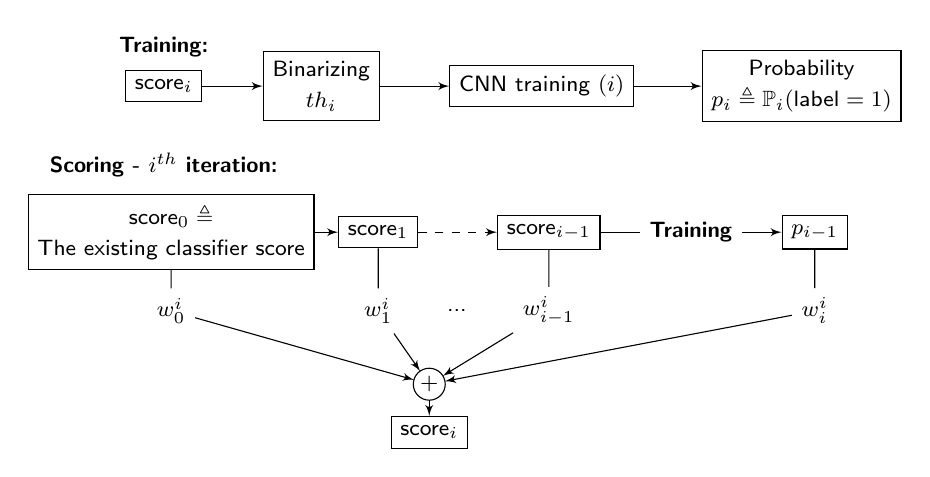
\begin{tikzpicture}[auto,>=latex',font=\sffamily\footnotesize,align=center]

                    \node (ph1) {\textbf{Training:}};
                    \node [state] (a1)[below of=ph1, node distance=.5cm] {$\text{score}_i$};
                    \node [state] (b1)[right of =a1, node distance=2cm] {Binarizing\\$th_i$};
                    \node [state] (c1)[right of =b1, node distance=2.8cm] {CNN training $(i)$};
                    \node [state] (d1)[right of =c1, node distance=3.3cm] {Probability\\$p_i\triangleq\p_i(\text{label}=1)$};

                    \node (ph2)[below of=a1, node distance=1cm] {\textbf{Scoring - $i^{th}$ iteration:}};
                    \node [state] (a) [below right=.1cm and -3.3cm of ph2]{$\text{score}_0\triangleq$\\The existing classifier score};
                    \node [state] (b) [right=.3cm of a]{$\text{score}_1$};
                    \node [state] (c) [right=1cm of b]{$\text{score}_{i-1}$};
                    \node (cc) [right=.5cm of c]{\textbf{Training}};
                    \node [state] (d) [right=.5cm of cc]{$p_{i-1}$};

                    
                    \node (w0) [below of=a] {$w_0^i$};
                    \node (w1) [below of=b] {$w_1^i$};
                    \node (wi1) [below of=c] {$w_{i-1}^i$};
                    \node (wi) [below of=d] {$w_i^i$};
                    \node (dots) [right of=w1] {...};
                    \node [sum] (e) [below right=.5cm and .2cm of w1] {$+$};
                    \node [state] (ee) [below =.2cm of e] {$\text{score}_i$};
                    \draw [->] (a) edge (b) (a1) edge (b1) (b1) edge (c1) (c1) edge (d1);
                    \draw [dashed,->] (b) edge (c);
                    \draw [->] (c) -- (cc) -- (d);
                    \draw [->](a) -- (w0) -- (e);
                    \draw [->](b) -- (w1) -- (e);
                    \draw [->](c) -- (wi1) -- (e);
                    \draw [->](d) -- (wi) -- (e);
                    \draw [->] (e) --(ee);
                \end{tikzpicture}
                \caption{Relabelling strategy}
            \end{figure}
			%[x] notation w_{i,j}
        \paragraph{2-moving average: $\forall i\:[w_i^i=w_{i-1}^i=1/2\text{  and } w^i_j=0, \forall j\in\llbracket 0,i-2\rrbracket]$}: In this case we only consider the previous score and the CNN training score to relabel the samples. Right after the first iteration we improve the overall performance by around 2\%. After 7 iterations, we notice that the performance (average precision and AUC) is not monotonically improving (figure \ref{perfBoot}: bootstrap 1 and figure \ref{roc:bs1}). One possible interpretation is that some informative hard examples are sensitive to bootstrapping and they keep changing sides after each iteration e.g. the $4^{\text{th}}$ and $9^{\text{th}}$ image in figure \ref{bs2:pos}

        \paragraph{Average, $\forall i\:[\forall j\in\llbracket 0,i\rrbracket,\:w_j^i=\frac{1}{i+1}]$}: Now we consider all the previous scores plus the CNN training score to relabel the samples. This tends to stabilize the relabelling as we are less dependent on a single CNN training. After few iterations we can give more confidence to the CNN score by going back to the 2-moving average (starting from iteration 5).
        Again the performance is fluctuating but it's still improving upon the bootstrapping with the 2-moving average (figure \ref{perfBoot}: bootstrap 2 and figure \ref{roc:bs2}). 
            \begin{figure}[H]
                \centering
                \includegraphics[width=13cm]{exp4/ap_auc_2}
                \caption{Performance improvement at each iteration of bootstrapping\label{perfBoot}}
            \end{figure}
            \begin{figure}[H]
                \centering
                \subfloat[ROC - bootstrap 1\label{roc:bs1}]{\includegraphics[height=5cm]{exp4/roc}}
                \subfloat[PR - bootstrap 1]{\hspace{10pt}\includegraphics[height=5cm]{exp4/pr}}
                \subfloat[ROC - bootstrap 2\label{roc:bs2}]{\hspace{10pt}\includegraphics[height=5cm]{exp4/roc2}}\\
                \subfloat[PR - bootstrap 2]{\includegraphics[height=5cm]{exp4/pr2}}
                \subfloat[ROC - comparison]{\hspace{10pt}\includegraphics[height=4.8cm]{exp4/roc_log_b1vb2}}
                \subfloat[PR - comparison]{\hspace{10pt}\includegraphics[height=5cm]{exp4/prb1vb2}}
                \caption{Performance at each bootstrap iteration : bootstrap 1\&2}
            \end{figure}
            %[x]remettre la meilleure courbe du bootstrap précédent.
        %[x] Mettre des images de cas difficiles pour le bootstrap
        \paragraph{}
        Some samples from the training set are difficult to label and after multiple bootstrap iterations the model fails to reveal their true label, the bootstrap scores are either fluctuating around the decision threshold or completely outside the desired domain.
        %[ ] à clarifier + lier images et graphes
        \begin{figure}[H]
        \begin{minipage}{.3\textwidth}
        \vspace{-40pt}
        \includegraphics[width=4cm]{exp4/bs1_images_neg}
        \end{minipage}\hspace{-20pt}
        \begin{minipage}{.3\textwidth}
        \subfloat[Scores - bootstrap 1]{\includegraphics[width=6cm]{exp4/bs1_scores_neg}}\\
        \subfloat[Probabilities - bootstrap 1]{\includegraphics[width=6cm]{exp4/bs1_probas_neg}}
        \end{minipage}\hspace{30pt}
        \begin{minipage}{.3\textwidth}
        \subfloat[Scores - bootstrap 2]{\includegraphics[height=2.2cm]{exp4/bs2_scores_neg}}\\
        \subfloat[Probabilities - bootstrap 2]{\includegraphics[height=2.2cm]{exp4/bs2_probas_neg}}
        \end{minipage}
        \caption{Negative samples - scores and probabilities at each bootstrap iteration\label{bs2:neg}}
        \end{figure}
        
        \begin{figure}[H]
        \begin{minipage}{.3\textwidth}
        \vspace{-40pt}
        \includegraphics[width=4cm]{exp4/bs1_images_pos}
        \end{minipage}\hspace{-20pt}
        \begin{minipage}{.3\textwidth}
        \subfloat[Scores - bootstrap 1]{\includegraphics[width=6cm]{exp4/bs1_scores_pos}}\\
        \subfloat[Probabilities - bootstrap 1]{\includegraphics[width=6cm]{exp4/bs1_probas_pos}}
        \end{minipage}\hspace{30pt}
        \begin{minipage}{.3\textwidth}
        \subfloat[Scores - bootstrap 2]{\includegraphics[height=2.2cm]{exp4/bs2_scores_pos}}\\
        \subfloat[Probabilities - bootstrap 2]{\includegraphics[height=2.2cm]{exp4/bs2_probas_pos}}
        \end{minipage}
        \caption{Positive samples - scores and probabilities at each bootstrap iteration\label{bs2:pos}}
        \end{figure}
	\subsubsection*{Extension}
	Instead of relying on the scores of the old classifier for the initial labeling, we can try to use our best classifier, \texttt{PerfTr3}, to perform the initial annotation, before bootstraping with the \emph{Average} method described above. As the initial classification is much better than the old classifier, the performances obtained are much better than in the previous section. Due to the initial labelling, the network is more prone to overfitting, and we had to limit the training phase to 5000 iterations to avoid a strong decrease in performances.
	 	Yet, we succeeded in obtaining a better accuracy than \texttt{PerfTr3} after three iterations.
	 	 \begin{figure}[H]
                \centering
                \includegraphics[width=10cm]{bootstraphk/acc}
                \includegraphics[width=10cm]{bootstraphk/auc}
                \caption{}
         \end{figure}
         Overall, the Area Under Curve indicator remains close to the initial performance of \texttt{PerfTr3}. Even if the gain in performance is small in absolute, compared to the advance obtained when starting the bootstrap with noisy labels (curve \emph{Boot2}) we still get a significant relative increase in performances compared to the \texttt{PerfTr3} results. In the table \ref{tableperfcomp}, we see how for small false positive rates (below 0.1) the improvement brought by the bootstrap over the simple \texttt{PerfTR3} CNN is significative, peaking at a 55\% improvement of the true positive rate after three iterations. The instability of the CNN over the iterations is also apparent: after four iterations the improvement over the baseline decreases, maybe caused by an overfitting.
          \begin{figure}[H]
                \centering
                \subfloat[ROC]{\includegraphics[height=6cm]{bootstraphk/roczoom_withb2}}
                \subfloat[log-ROC]{\includegraphics[height=6cm]{bootstraphk/logroc_withb2}}\\
          	    \begin{minipage}{.45\textwidth}
                \subfloat[PR]{\includegraphics[height=6cm]{bootstraphk/pr_withb2}}
                \end{minipage}
                \begin{minipage}{.4\textwidth}
                    \subfloat[Compared performances at 0.05 false pos. rate \label{tableperfcomp}]{
							\begin{tabular}{|l|l|l|}
                				\hline
                				CNN & True pos. rate & \% improv. \\ \hline
                				PerfOld & 0.7358 & - \\ \hline
                				PerfTr3 & 0.9820 & 0\% \\ \hline
                				It 1 & 0.9756 & -35.5\%  \\ \hline
                				It 2 & 0.9837 & 9.5\%  \\ \hline
                				It 3 & 0.9919 & 55.0\%  \\ \hline
                				It 4 & 0.9878 & 32.3\%  \\ \hline
                				It 5 & 0.9715 & -58.3\%  \\ \hline
                				It 6 & 0.9715 & -58.3\%  \\ \hline
                				It 7 & 0.9756 & -35.5\%  \\ \hline
		                        \end{tabular}}
            \end{minipage}
			\caption{Performance at each bootstrap iteration}
          \end{figure}
          Finally we display selected examples of pictures from the test set where the CNN is uncertain : the classification of those images oscillates from an iteration to the next. The pictures that should be labelled positive are similar to some exhibited before, where the glasses are either extremely thin, or where the central junction of the glasses is not clearly visible. 
          The negative pictures also exhibit examples of unexpected poses (facial orientation), light effects or eyebrows that still disturbs the classifier even if it is not relying on the knowledge of the old classifier.
       \begin{figure}[H]
        \begin{minipage}{.3\textwidth}
        \includegraphics[height=4.5cm]{bootstraphk/zerosfaces}
        \end{minipage}
        \begin{minipage}{.55\textwidth}
         \subfloat[Probabilities $\p(label=1)$ at every bootstrap iteration]{\includegraphics[height=3cm]{bootstraphk/zeros}}
        \end{minipage}
        \caption{Negative samples (test set)}
        \end{figure}
        \begin{figure}[H]
        \begin{minipage}{.3\textwidth}
        \includegraphics[height=4.5cm]{bootstraphk/onesfaces}
        \end{minipage}
        \begin{minipage}{.55\textwidth}
        \subfloat[Probabilities $\p(label=1)$ at every bootstrap iteration]{\includegraphics[height=3cm]{bootstraphk/ones}}
        \end{minipage}
        \caption{Positive samples (test set)}
        \end{figure}    
	 	By tracking the evolution of the scores of those images, it appears that at the beginning the bootstrap has a contractive action: when considering the negative labels, at the third iteration seven pictures over nine are correctly identified; the same behavior can be observed for positive labels at the fourth iteration, where six out of the nine pictures are correctly sorted. But those evolutions are not synced between both labels, and the scores are not stables in the following iterations. It is important to note that those pictures were selected for their variability from an iteration to the next and the scores evolution is thus generally worst than for a randomly selected image.
	\subsection{Noise prediction}\label{sec:cleansing}
            Instead of considering the problem as a binary classification we distinguish 4 different classes given the ground truth label of an image and the old classifier score. We train a CNN that takes the image as an input, and output a label $i\in\llbracket0,3\rrbracket$ that expresses if this picture would be a true positive, false positive, true negative or false negative when using the old classifier on it. During the supervised training phase, both the ground truth and the old classifier results are used to generate the labels $i$.
            
            The CNN classifier, trained on a hand labelled dataset (\texttt{Tr1}), will help uncover the noisy labels in order to train a robust model on the cleansed labels. We tested this method with $t=30$ and $t=40$ where the training set has the following distributions:
            \begin{table}[H]
                \subfloat[Classes]{
                \begin{tabular}{c|c|c|}
                \cline{2-3}
                            &\multicolumn{2}{|c|}{truth}\\
                \cline{2-3}
                            & 0 & 1\\
                \hline
                \multicolumn{1}{|c|} {score $<$ th} &  c0  &  c1\\
                \hline
                \multicolumn{1}{|c|} {score $>$ th }&  c2  &  c3\\
                \hline
                \end{tabular}}
                \hspace{10pt}
                \subfloat[t=30]{
                \begin{tabular}{|c|c|c|}
                \hline
                class & \# training & \# test \\
                \hline
                noisy=true=0 & 3888 & 4349\\
                noisy=0 true=1 & 88 & 100\\
                noisy=1 true=0 & 50 & 66\\
                noisy=true=1 & 126  & 146\\
                \hline
                \end{tabular}
                }
                \subfloat[t=40]{
                \begin{tabular}{|c|c|c|}
                \hline
                class & \# training & \# test \\
                \hline
                noisy=true=0 & 3919 & 4394\\
                noisy=0 true=1 & 116 & 134\\
                noisy=1 true=0 & 19 & 21\\
                noisy=true=1 & 98  & 112\\
                \hline
                \end{tabular}
                }
                \caption{Training \& test set statistics when thresholding at t=30 and at t=40}
            \end{table}
            \begin{figure}[H]
            \centering
            \includegraphics[width=7cm]{isnoisy/roc_multiclass_30}
            \includegraphics[width=7cm]{isnoisy/roc_multiclass_40}
            \caption{Multiclass ROC curves}
            \end{figure}
            The model is unable to expose the false positives, which is quite expected seeing the dataset skewness, and most samples of class 2 end up in class 0. This fact is more pronounced  with $t=40$. In the context of labels cleansing this is harmless as both classes will lead to the same correction.
            \begin{figure}[H]
            \centering
            \hspace{40pt}
            \begin{minipage}{.2\textwidth}
            \vspace{30pt}
            \subfloat[Classes]{
                \resizebox{\textwidth}{!}{%
                \begin{tabular}{|c|c|c|}
    					\hline
    					Class & Truth & Old label \\ \hline
    					0     & 0            & 0              \\ \hline
    					1     & 1            & 0              \\ \hline
    					2     & 0            & 1              \\ \hline
    					3     & 1            & 1              \\ \hline
    				\end{tabular}%
    			}}
			\end{minipage}
            \hspace{10pt}\begin{minipage}{.6\textwidth}
            \subfloat[t=30]{\includegraphics[height=3cm]{isnoisy/cfmat30}}
            \hspace{10pt}\subfloat[t=40]{\includegraphics[height=3cm]{isnoisy/cfmat40}}
            \end{minipage}
            \caption{Confusion matrices}
            \end{figure}
            In the misclassified images (in the sense where the corrected label is different from the ground truth label) we notice that the same issues encountered before persist namely the difficulty to detect rimless glasses or handle unusual poses (figure \ref{fig:flipped}). On the bright side, with all the labels flipped we can reach an accuracy of 98.8\% with the model learned from cleansed labels originally thresholded at $t=40$.
            
            \begin{figure}[H]
            \centering
            \subfloat[Flipped labels t = 30]{\includegraphics[height=2cm]{isnoisy/flip_pos_th30}\includegraphics[height=2cm]{isnoisy/flip_neg_th30}}
            \hspace{20pt}
            \subfloat[Misclassified t = 30]{\includegraphics[height=2cm]{isnoisy/mis_pos_th30}\includegraphics[height=2cm]{isnoisy/mis_neg_th30}}
            \\
            \subfloat[Flipped labels t = 40]{\includegraphics[height=2cm]{isnoisy/flip_pos_th40}\includegraphics[height=2cm]{isnoisy/flip_neg_th40}}
            \hspace{20pt}
            \subfloat[Misclassified t = 40]{\includegraphics[height=2cm]{isnoisy/mis_pos_th40}\includegraphics[height=2cm]{isnoisy/mis_neg_th40}}
            
            \caption{Extract from the test set\label{fig:flipped}}
            \end{figure}
            After rectifying the labels we run the baseline (softmax loss) on the full training set \texttt{CASIA} $\approx 382k$ images. Although thresholding at $t=40$ gave poor performances compared to other thresholds (c.f. \ref{vary:th}) it's more prone to noise prediction with more false negatives that the model has proven to deal with successfully and less false positives harder to unmask (figure \ref{per:isnoisy}).
            \begin{figure}[H]
            \centering
            \subfloat[t=40]{\includegraphics[height=5.5cm]{isnoisy/pred40}}
            \subfloat[comparison]{\includegraphics[height=5.5cm]{isnoisy/pred}}
            \subfloat[comparison log-scale]{\includegraphics[height=5.5cm]{isnoisy/pred_log}}
            \caption{Performances improvement: for $t=30$ and $t=40$, baseline model on noisy labels compared to the model with cleansed labels. $it=0$ extension is the first bootstrap iteration when labelling the full training set with \texttt{perfTr3}. This first iteration could be seen as cleansing the labels with a binary classifier trained on clean labels (\texttt{Tr3})\label{per:isnoisy}}
            \end{figure}

\section{Testing}
    In order to assess the performances of our models independently from the \texttt{CASIA} dataset specificities, we tested it on other datasets with similar samples. We compare the performances of the old classifier with three of our models:
    \begin{itemize}
    	\item the model trained on the hand-labelled set \texttt{Tr3} with the infogain loss, denoted \texttt{M1}.
    	\item the model learned by bootstrapping (5 iterations) on the noisy dataset, using the \emph{average} update rule,  denoted \texttt{M2}.
    	\item the model learned by bootstrapping (3 iterations) on \texttt{CASIA} initially relabelled with \texttt{PerfTr3} with the same \emph{average} update rule, denoted \texttt{M3}.
    \end{itemize}
    The pictures in each of the datasets used are in a similar form-factor as the ones in \texttt{CASIA}, and have the following characteristics:
   
	\begin{table}[H]
	\centering
	\begin{tabular}{|l|l|l|l|l|}
	\hline
	Base & \#samples & \#positive samples & positive ratio & Specificities                                  \\ \hline
	B1   & 807       & 146       &   18.7\%     & All poses, no expressions, mainly caucasian.   \\ \hline
	B2   & 2000      & 90     &      4.5\%      & Fixed pose, few expressions.                   \\ \hline
	B3   & 5000      & 332    &       6.6\%     & Fixed pose, few expressions, mainly caucasian. \\ \hline
	\end{tabular}
	\caption{Characteristics of the test bases.}
	\end{table}
	On the first set, as shown in figure \ref{fig:BB1}, we obtain results similar to those seen while validating our models: the models learnt on clean subsets perform better, while the bootstrap learned on the noisy set performs halfway between those and the old classifier. Results on the two other sets (resp. figures \ref{fig:BB2} and \ref{fig:BB3}) are much harder to interpet due to the repartition of data. Nevertheless both M1 and M3 always perform better than the old classifier baseline. The M2 model is probably more sensitive to the specificities of each dataset as it relies on the scores of the old classifier. Overall, those tests allowed us to validate our models on other similar datasets, showing that the CNN did not overfit during the learning phase and succeeded in capturing significant features of the images.
	
    \begin{figure}[H]
                \centering
                \subfloat[ROC]{\includegraphics[width=150px]{testbases/roc_B53}}
                \subfloat[ROC (zoom)]{\includegraphics[width=150px]{testbases/roc_zoom_B53}}
				\subfloat[log-ROC]{\includegraphics[width=150px]{testbases/logroc_B53}}
                 \caption{Results on B1}
                 \label{fig:BB1}
                \subfloat[ROC]{\includegraphics[width=150px]{testbases/roc_B61}}
                \subfloat[ROC (zoom)]{\includegraphics[width=150px]{testbases/roc_zoom_B61}}
                \subfloat[log-ROC]{\includegraphics[width=150px]{testbases/logroc_B61}}
                \caption{Results on B2}
                \label{fig:BB2} 
                \subfloat[ROC]{\includegraphics[width=150px]{testbases/roc_B64}}
                 \subfloat[ROC (zoom)]{\includegraphics[width=150px]{testbases/roc_zoom_B64}}
                \subfloat[log-ROC]{\includegraphics[width=150px]{testbases/logroc_B64}}
                \caption{Results on B3}
                \label{fig:BB3}
    \end{figure} 
    

%[x] to finish 
\section{Conclusion}
    Through this project, we studied multiple methods, from pre-processing the data to modifying the CNN learning phase. Overall, the best solution performance-wise remains to use a hand-labelled small subset: our best results were obtained by labelling less than 2\% of the \texttt{CASIA} dataset. Classical performance enhancement techniques such as bootstrapping have shown to be very efficient on both clean and noisy datasets, improving accuracy and precision.\\
    Models that take into account (either in the classifier or via another CNN) the dependence between the noise and the content of the pictures in more refined ways are still limited to cases constrained by heavy assumptions on the noise type and distribution, but remain promising; literature on this topic will surely be expanded in the coming years, as research progresses.\\
    When focusing on usability of the studied methods, aside from the manual hand-labelling option, the error-prediction experiment appears as extremely interesting in the sense that it can be plugged into an existing data processing pipeline.


%[x] to finish (S) 
\section{Acknowledgments}
    We would like to thank our supervisor, C. Herold, along with S. Gentric and V. Despiegel at Morpho, for guiding us during the whole project, taking the time to answer our questions, helping us with our results and proof-reading this report. We also thank J. Milgram and J. Bohn\'e from Morpho for their insightful remarks. Finally, we would like to thank the pedagogic team at Centrale, especially N. Paragios for his supervision and L. Series for helping us with all technical matters related to Caffe. 
%[x] to finish (S) 
\section{Appendices}
\subsection{Hyperparameters of the CNN}{\label{cnn_param}}
Configuration file used to set up the CNN in Caffe.
\begingroup
\obeylines
\verbatiminput{solver.prototxt}
\endgroup

\subsection{Other experiments}
 Other peripheral experiments were made during our study. We shortly describe them below, along with the obtained results.
        \subsubsection{General run time}
            Our first test was devoted to finding which number of iterations should be necessary in order for our network to stabilize. We thus started by letting the training phase run for 150k iterations. As the results exhibited overfitting and by tracking the evolution of accuracy and AUC, we settled for an ideal number of iterations of 10k. This corresponds to a run time of 20 to 25 minutes on a single Nvidia K40 GPU card. We also generally extracted the results at 5k and 20k iterations for most of our runs, in order to detect variations of performance in different experiments.
        %[x]give learning time on size
        \subsubsection{Color vs gray}
        	Another early experiment was performed in order to assess the importance of using RGB pictures instead of gray levels pictures. A test led on the \texttt{Tr2} base and validated on the \texttt{Test} set gives AUCs of 0.991 and 0.982 for RGB and Gray levels respectively. The difference brought by keeping the three channels of the images is thus non-negligible ; this confirms the fact that the gain in information brought by having access to the color (and not only the luminance) is useful for detecting (an absence of) glasses in some pictures.
            \begin{figure}[H]
            \centering
            \subfloat[ROC curves (zoom)]{\includegraphics[height=4.5cm]{figures/rgb_gray/roc_hk.pdf}}
            \vspace{5pt}
            \subfloat[Precision-Recall curves]{\includegraphics[height=4.5cm]{figures/rgb_gray/pr_hk.pdf}}
            \subfloat[ROC log curves]{\includegraphics[height=4.5cm]{figures/rgb_gray/roc_log_hk.pdf}}
            \end{figure}
            %\begin{figure}[H]
            %    \centering
            %    \subfloat[ROC curves]{\includegraphics[width=5cm]{figures/rgb_gray/roc_rgbgray.pdf}}
            %    \vspace{5pt}
            %    \subfloat[Precision-Recall curves]{\includegraphics[width=5cm]{figures/rgb_gray/recall_rgbgray.pdf}}
            %\end{figure}

\bibliographystyle{unsrt}
\bibliography{Refs}
\end{document}